\documentclass[12pt,a4paper]{article}

\usepackage[utf8]{inputenc}
\usepackage[T1]{fontenc}
\usepackage[slovak]{babel}
\usepackage{geometry}
\usepackage{booktabs}
\usepackage{array}
\usepackage{amsmath}
\usepackage{graphicx}
\usepackage[section]{placeins}
\usepackage{hyperref}
\usepackage[numbers,sort&compress]{natbib}

\geometry{margin=2.5cm}
\hypersetup{
  colorlinks=true,
  linkcolor=black,
  citecolor=black,
  urlcolor=blue
}
\emergencystretch=3em

\title{Fuzzy expertný systém na prioritizáciu Z-DNA-formujúcich regiónov}
\author{Ing. Michal Petrovič}
\date{2026}

\begin{document}
\maketitle

\begin{abstract}
Seminárna práca rieši problém podpory rozhodovania pri výbere kandidátnych Z-DNA-formujúcich regiónov pre experimentálnu validáciu alebo manuálnu kuráciu. Riešenie je navrhnuté ako univerzálna rozhodovacia vrstva použiteľná nad kandidátmi z ľubovoľného referenčného genómu, pokiaľ sú dostupné sekvenčné skóre a základné anotačné príznaky. Vstup \texttt{zdna\_score} je normalizovaný do intervalu 0 až 1 a kandidátne regióny majú dĺžku 8 až 400 bp. Implementácia v jazyku Python porovnáva sedem rozhodovacích stratégií: jednoduchý baseline, sekvenčný konsenzus, vážený lineárny model, tri Mamdaniho fuzzy iterácie a Takagiho-Sugenov fuzzy model. Benchmark obsahuje 320 kandidátov rozdelených na tréningovú, validačnú a testovaciu časť v pomere 192/64/64. Najlepší model bol vybraný na validačnom splite a vyhodnotený na oddelenom testovacom splite, kde dosiahol MAE 5,15, Spearmanovu koreláciu 0,944, zhodu rozhodovacej fronty 0,766 a kompozitný index kvality 82,59. Práca dopĺňa ablačnú analýzu vstupov, odhad intervalovej neistoty a externé overenie na reálnych per-locus overlay dátach zo Shin et al. \citep{shin2016}.
\end{abstract}

\section{Zadanie seminárnej práce}

Navrhované zadanie seminárnej práce je: \emph{navrhnúť, implementovať a experimentálne overiť fuzzy expertný systém pre prioritizáciu kandidátnych Z-DNA-formujúcich regiónov v genómových dátach}. Praktickým cieľom nie je dokázať, že konkrétny región in vivo tvorí Z-DNA, ale rozhodnúť, ktoré kandidáty majú dostať prednosť pri validácii, manuálnej kontrole alebo ďalšej bioinformatickej analýze.

Rozhodovací problém vzniká preto, že výpočtové nástroje môžu vytvoriť veľké množstvo kandidátnych regiónov, zatiaľ čo experimentálna validácia je obmedzená časom, nákladmi a dostupnosťou laboratórnych kapacít. Samotné sekvenčné skóre nestačí: kandidát môže mať silný Z-DNA motív, ale zároveň sa môže nachádzať v repetitívnej oblasti, ďaleko od regulačného kontextu alebo môže pochádzať iba z jednej proxy evidencie. Naopak, kandidát so stredným sekvenčným skóre môže byť zaujímavý, ak sa nachádza v promótore, v blízkosti TSS alebo v CpX bohatom prostredí.

\section{Biologické a metodické východiská}

Z-DNA je alternatívna ľavotočivá konformácia DNA. Jej tvorba závisí od sekvenčného zloženia, superhelikálneho napätia a regulačného kontextu. Prehľadová literatúra zdôrazňuje, že Z-DNA a Z-RNA štruktúry majú dynamickú a kontextovo závislú úlohu v genóme \citep{umerenkov2023}. Experimentálne mapované Z-DNA lokality boli asociované s aktívne transkribovanými oblasťami \citep{shin2016}. Pri interpretácii výpočtových predikcií je preto potrebné rozlišovať medzi sekvenčnou predispozíciou a funkčnou aktivitou v bunke.

Ako sekvenčný zdroj rozhodovania slúži normalizované \texttt{zdna\_score}, ktoré reprezentuje intenzitu Z-DNA-formujúceho signálu v rozsahu 0 až 1. Tento vstup môže pochádzať z heuristického nástroja typu Z-DNA Hunter \citep{petrovic2025}. Druhou sekvenčnou vrstvou je pravdepodobnosť modelu podobného DNABERT prístupu, teda sequence-only modelu pracujúceho s DNA tokenmi \citep{ji2021}. CpX kontext je motivovaný nástrojmi na identifikáciu CpG, CpA, CpT a CpC ostrovčekov \citep{bartas2025}. V tejto práci sa nepoužíva bunkovo špecifická multi-omics pravdepodobnosť; cieľom je rozhodovacia vrstva použiteľná už po sekvenčnej a anotovanej genómovej analýze.

\section{Teoretické východiská fuzzy rozhodovania}

Fuzzy množiny zaviedol Zadeh ako formalizáciu neurčitosti pomocou stupňov príslušnosti v intervale $[0,1]$ \citep{zadeh1965}. Tento prístup je vhodný pre rozhodovanie, kde ostré hranice pôsobia umelo. V tejto úlohe napríklad nie je prirodzené tvrdiť, že kandidát so skóre 0,699 je nízky a kandidát so skóre 0,700 je vysoký.

Prvá skupina modelov používa Mamdaniho inferenčný mechanizmus s pravidlami typu \emph{ak--potom}, max-min agregáciou a defuzzifikáciou výslednej fuzzy množiny \citep{mamdani1975}. Druhá fuzzy alternatíva používa Takagiho-Sugenov model, v ktorom konsekvent pravidla nie je fuzzy množina, ale numerická lokálna funkcia \citep{takagi1985}. Mamdaniho model je transparentnejší pri vysvetľovaní pravidiel, zatiaľ čo Takagiho-Sugenov model je vhodnejší na numerickú kalibráciu a porovnanie s lineárnym baseline.

\section{Vstupné premenné a výstup}

Rozhodovacou jednotkou je kandidátny Z-DNA-formujúci región v referenčnom genóme. Každý kandidát má dĺžku 8 až 400 bp a je opísaný skupinou znakov:

\begin{itemize}
  \item \texttt{zdna\_score}: normalizované skóre Z-DNA signálu v rozsahu 0 až 1,
  \item \texttt{z\_dnabert\_probability}: pravdepodobnosť sekvenčného modelu v rozsahu 0 až 1,
  \item \texttt{cpx\_overlap\_pct}: percentuálny prekryv kandidáta s CpX ostrovčekom,
  \item \texttt{tss\_distance\_bp}: vzdialenosť od najbližšieho TSS,
  \item \texttt{promoter\_overlap} a \texttt{regulatory\_marks}: regulačný kontext,
  \item \texttt{repeat\_overlap\_pct}: podiel repetitívneho prekryvu,
  \item \texttt{independent\_support}: podpora nezávislou vrstvou v rámci toho istého druhu,
  \item \texttt{primer\_uniqueness} a \texttt{length\_bp}: praktická validovateľnosť.
\end{itemize}

Pre fuzzy inferenciu sú všetky odvodené premenné prevedené do škály 0 až 100. Normalizované \texttt{zdna\_score} sa teda násobí stomi. Dĺžková zložka validovateľnosti používa trapézovú funkciu s plnou príslušnosťou v intervale 8 až 400 bp. Tento rozsah pokrýva krátke 8 bp výstupy Z-DNA Hunter aj 384 bp lokusy Shin validačného datasetu.

\begin{figure}[htbp]
\centering
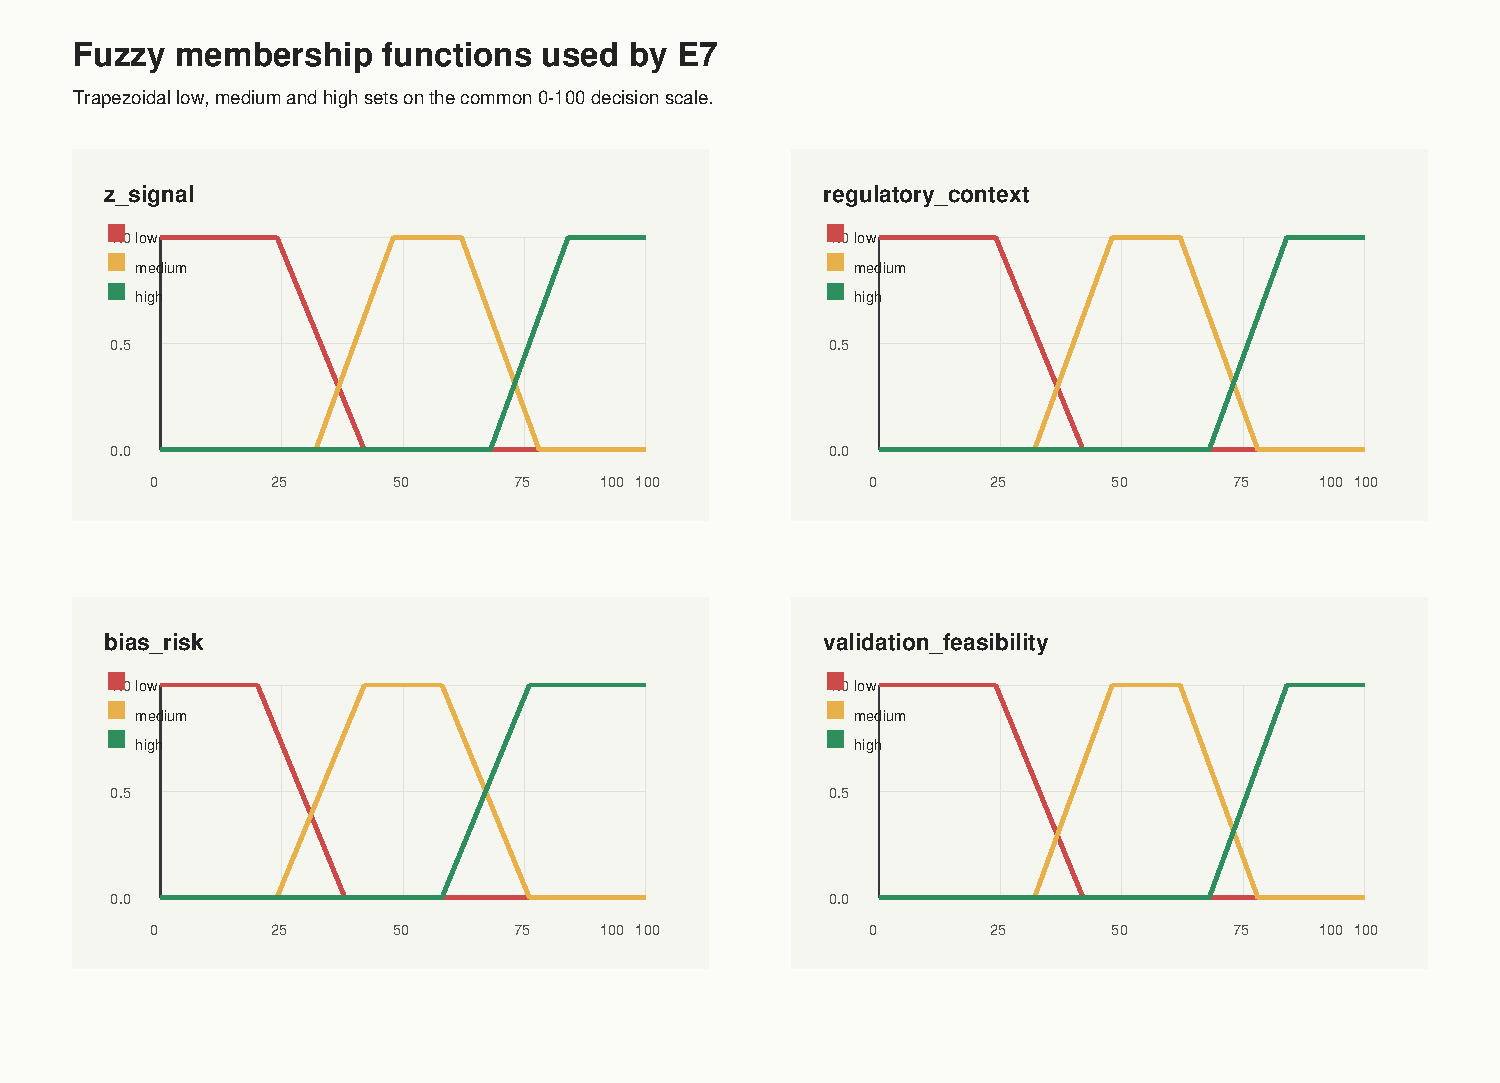
\includegraphics[width=\linewidth]{../outputs/membership_functions.pdf}
\caption{Funkcie príslušnosti použité vo finálnom modeli E7. Premenné \texttt{z\_signal}, \texttt{regulatory\_context} a \texttt{validation\_feasibility} používajú konzervatívne hranice nízkej, strednej a vysokej hodnoty; \texttt{bias\_risk} má samostatné hranice, pretože vysoká hodnota predstavuje penalizačný signál.}
\end{figure}

Výstupom je spojité skóre priority a štyri rozhodovacie fronty:

\begin{itemize}
  \item \texttt{A\_validovat}: kandidát vhodný pre prvú vlnu validácie,
  \item \texttt{B\_prioritne\_preskumat}: kandidát vhodný na bližšiu analýzu,
  \item \texttt{C\_manualna\_kuracia}: kandidát vyžadujúci manuálnu kontrolu,
  \item \texttt{D\_odlozit}: nízka priorita alebo vysoké riziko biasu.
\end{itemize}

\section{Návrh pravidlovej bázy}

Mamdaniho systém je navrhnutý hierarchicky. Namiesto jedného veľkého pravidlového systému s piatimi vstupmi sa rozhodovanie rozdelí na tri vrstvy: biologická plausibilita, dôveryhodnosť evidencie a finálna priorita. Pri troch jazykových hodnotách na päť vstupných premenných by úplná pravidlová báza obsahovala $3^5 = 243$ pravidiel. Hierarchické riešenie používa 33 Mamdaniho pravidiel a vo finálnej kalibrovanej verzii E6 ešte 9 prahových korekcií.

\begin{table}[htbp]
\centering
\caption{Štruktúra Mamdaniho pravidlovej bázy.}
\begin{tabular}{>{\raggedright\arraybackslash}p{3.0cm}>{\raggedright\arraybackslash}p{3.0cm}>{\raggedright\arraybackslash}p{2.4cm}>{\raggedright\arraybackslash}p{3.2cm}r}
\toprule
Vrstva & Vstupy & Výstup & Úloha & Pravidlá \\
\midrule
Biologická plausibilita & signál, kontext & plausibilita & biologický význam & 9 \\
Dôvera v evidenciu & evidencia, bias & dôvera & metodická spoľahlivosť & 9 \\
Finálna priorita & plausibilita, dôvera, validácia & priorita & rozhodovacia fronta & 15 \\
Kalibrácia E6 & odvodené prahy & skóre & oprava reziduí & 9 \\
\bottomrule
\end{tabular}
\end{table}

Prvá vrstva kombinuje \texttt{z\_signal} a \texttt{regulatory\_context}. Obsahuje úplnú kombináciu hodnôt nízka, stredná a vysoká pre dve vstupné premenné. Pravidlo B1 hovorí, že vysoký Z-DNA signál vo vysokom regulačnom kontexte vedie na vysokú biologickú plausibilitu. Pravidlo B5 drží vysoký sekvenčný signál bez kontextu iba na strednej plausibilite. Pravidlo B7 odkladá kandidáta, ak je nízky signál aj kontext.

Druhá vrstva kombinuje \texttt{evidence\_support} a \texttt{bias\_risk}. Pravidlo C1 dáva silnú dôveru kombinácii vysokej evidencie a nízkeho biasu. Pravidlo C3 je v konzervatívnej iterácii prísne: vysoký bias oslabuje aj vysokú evidenciu. Pravidlo C6 označuje strednú evidenciu pri vysokom biase ako slabú.

Tretia vrstva používa 15 pravidiel. Nepokrýva mechanicky všetkých 27 kombinácií, pretože viaceré kombinácie majú rovnaký rozhodovací význam. Pravidlo P1 posiela kandidáta s vysokou plausibilitou, silnou dôverou a vysokou validovateľnosťou do kritickej priority. Pravidlá P5 a P14 bránia tomu, aby kandidát s nepresvedčivou evidenciou alebo nízkou validovateľnosťou automaticky skončil v prvej validačnej vlne. Pravidlá P11 až P13 pokrývajú odkladové prípady so slabou plausibilitou, slabou evidenciou alebo nízkou realizovateľnosťou.

\subsection{Iterácie pravidiel}

Experimenty E4 až E6 používajú rovnakú hierarchickú štruktúru, ale menia hranice fuzzy množín a vybrané pravidlá. E4 je permissívna verzia: širšie interpretuje vysoký signál a pravidlo B3 považuje stredný Z-DNA signál vo vysokom kontexte za vysokú plausibilitu. E5 sprísňuje hranice vysokej množiny, B3 vracia iba strednú plausibilitu a C3 silnejšie penalizuje vysoký bias. E6 zachováva konzervatívnu bázu a pridáva 9 korekcií, ktoré penalizujú motívové kandidáty s vysokým biasom, obmedzujú kandidátov typu \texttt{model\_only} bez nezávislej evidencie a mierne zvyšujú prioritu sequence-only kandidátov s nízkym biasom a dobrou validovateľnosťou.

Model E7 je Takagiho-Sugenov variant. Používa rovnaké odvodené vstupy a 10 lokálnych pravidiel. Pravidlá TS1 až TS4 opisujú silný signál v silnom alebo strednom kontexte, TS5 pokrýva silný signál bez kontextu, TS7 a TS8 penalizujú vysoký bias a nízku validovateľnosť a TS9 odkladá kandidáta so slabým signálom aj kontextom. Konsekventy sú numerické lokálne priority a sú kombinované s lineárnym základom, takže E7 slúži ako numericky kalibrovaný fuzzy model s auditovateľnými lokálnymi pravidlami.

\section{Implementácia}

Implementácia je v súbore \path{src/zfr_fuzzy_expert.py}. Program implementuje trapézové funkcie príslušnosti, Mamdaniho max-min inferenciu, agregáciu pravidiel maximom a defuzzifikáciu metódou ťažiska:

\[
P_i = \operatorname{centroid}\left(\max_{r \in R} \min(\alpha_r, \mu_{C_r}(x))\right),
\]
kde $\alpha_r$ je aktivácia pravidla $r$, $\mu_{C_r}$ je funkcia príslušnosti konsekventu a $x$ je univerzum výstupnej premennej priority.

Vstupom je CSV súbor \path{data/sample_candidates.csv}. Benchmark obsahuje 320 kandidátov univerzálneho genómového datasetu, štyri typy evidencie, split \texttt{train}/\texttt{validation}/\texttt{test} a referenčné skóre \texttt{expert\_priority\_score}. Program generuje porovnanie experimentov, finálny ranking, audit pravidiel, ablačnú analýzu, intervalovú neistotu a grafické výstupy:

\begin{itemize}
  \item \path{outputs/experiment_summary.csv} a \path{outputs/experiment_details.csv},
  \item \path{outputs/priority_ranking.csv} a \path{outputs/rules_audit.txt},
  \item \path{outputs/rule_coverage_summary.csv},
  \item \path{outputs/ablation_summary.csv} a \path{outputs/uncertainty_summary.csv},
  \item \path{outputs/shin_real_evaluation.csv} a \path{outputs/shin_real_predictions.csv},
  \item \path{outputs/membership_functions.pdf},
  \item \path{outputs/experiment_quality.pdf}, \path{outputs/prediction_vs_expert.pdf},
  \item \path{outputs/ablation_impact.pdf}, \path{outputs/uncertainty_intervals.pdf},
  \item \path{outputs/shin_real_comparison.pdf} a \path{outputs/shin_validation_trajectory.pdf}.
\end{itemize}

Súbor \path{src/prepare_shin_real_validation.py} navyše pripravuje externý Shin validačný dataset \path{data/shin_real_candidates.csv}. Vychádza z per-locus overlay súborov v \path{data/shin_data}, ktoré obsahujú prekryvy experimentálne overených pozitívnych a negatívnych Shin intervalov s výstupmi Z-DNA Hunter \citep{shin2016}. Pre toto overenie sa ZDNABERT nepoužíva ako vstup modelu. Vybrané boli iba nastavenia Z-DNA Hunter: \texttt{model1\_10bp}, \texttt{model2\_10bp}, \texttt{model2\_8bp}, \texttt{model2\_8bp\_65perc} a \texttt{model2\_10bp\_60perc}. ZDNABERT zostáva uvedený len ako externý porovnávací riadok v tabuľke výsledkov. Pôvodné Shin lokusy sú načítané zo súborov \path{data/shin_data/shin_original_fasta}; kandidát je ukotvený v pôvodnom lokuse a jeho dĺžka sa odvodí podľa najsilnejšieho dostupného Hunter prekryvu. CpX kontext sa počíta z exportov \path{data/shin_data/cpxhunter_exports}, ktoré sú rozdelené podľa chromozómu a typu \texttt{cpa}/\texttt{cpc}/\texttt{cpg}/\texttt{cpt}. Vzdialenosť od najbližšieho TSS je počítaná zo súboru \path{data/shin_data/Hum_ENSEMBL52.sga} k odvodenému kandidátovi a vstupuje do výpočtu regulačného kontextu rovnakým spôsobom ako v hlavnom benchmarku.

\section{Experimentálne vyhodnotenie}

Benchmark bol rozdelený na tréningovú časť s 192 kandidátmi, validačnú časť so 64 kandidátmi a testovaciu časť so 64 kandidátmi. Tréningová časť slúžila na iteratívne nastavenie hraníc fuzzy množín a pravidiel, validačná časť na výber najlepšieho modelu a testovacia časť na finálne porovnanie. Všetky výsledky v tabuľkách nižšie sú reportované pre oddelený testovací split, ak nie je uvedené inak.

Porovnaných bolo sedem stratégií:

\begin{itemize}
  \item E1: baseline používajúci iba normalizované \texttt{zdna\_score},
  \item E2: sekvenčný konsenzus \texttt{zdna\_score} a Z-DNABERT pravdepodobnosti,
  \item E3: vážený lineárny model s penalizáciou biasu,
  \item E4: prvá permissívna Mamdaniho fuzzy iterácia,
  \item E5: konzervatívnejšia Mamdaniho fuzzy iterácia,
  \item E6: kalibrovaný hierarchický Mamdaniho model,
  \item E7: Takagiho-Sugenov fuzzy model s lokálnymi numerickými konsekventmi.
\end{itemize}

Presnosť bola meraná pomocou MAE, RMSE, Spearmanovej korelácie, presnosti zaradenia do rozhodovacej fronty, presnosti so susednou toleranciou a precision@top-$k$, kde $k$ je počet kandidátov označených referenciou ako \texttt{A\_validovat}. Konečný index kvality kombinuje koreláciu, presnosť fronty, top-$k$ presnosť a penalizáciu absolútnej chyby.

\begin{table}[htbp]
\centering
\caption{Testovacie porovnanie rozhodovacích stratégií.}
\small
\begin{tabular}{lrrrrr}
\toprule
Model & MAE & Spearman & Fronta & Top-$k$ & Index \\
\midrule
E1 \texttt{zdna\_score} & 18,54 & 0,085 & 0,328 & 0,263 & 10,33 \\
E2 sekvenčný konsenzus & 13,28 & 0,409 & 0,312 & 0,526 & 34,82 \\
E3 vážený lineárny model & 5,69 & 0,943 & 0,719 & \textbf{0,842} & 80,79 \\
E4 Mamdani permissive & 10,55 & 0,863 & 0,531 & 0,789 & 67,60 \\
E5 Mamdani conservative & 11,21 & 0,870 & 0,625 & 0,632 & 66,95 \\
E6 Mamdani calibrated & 8,84 & 0,904 & 0,594 & 0,737 & 71,88 \\
E7 Takagi-Sugeno & \textbf{5,15} & \textbf{0,944} & \textbf{0,766} & \textbf{0,842} & \textbf{82,59} \\
\bottomrule
\end{tabular}
\end{table}

\begin{figure}[htbp]
\centering
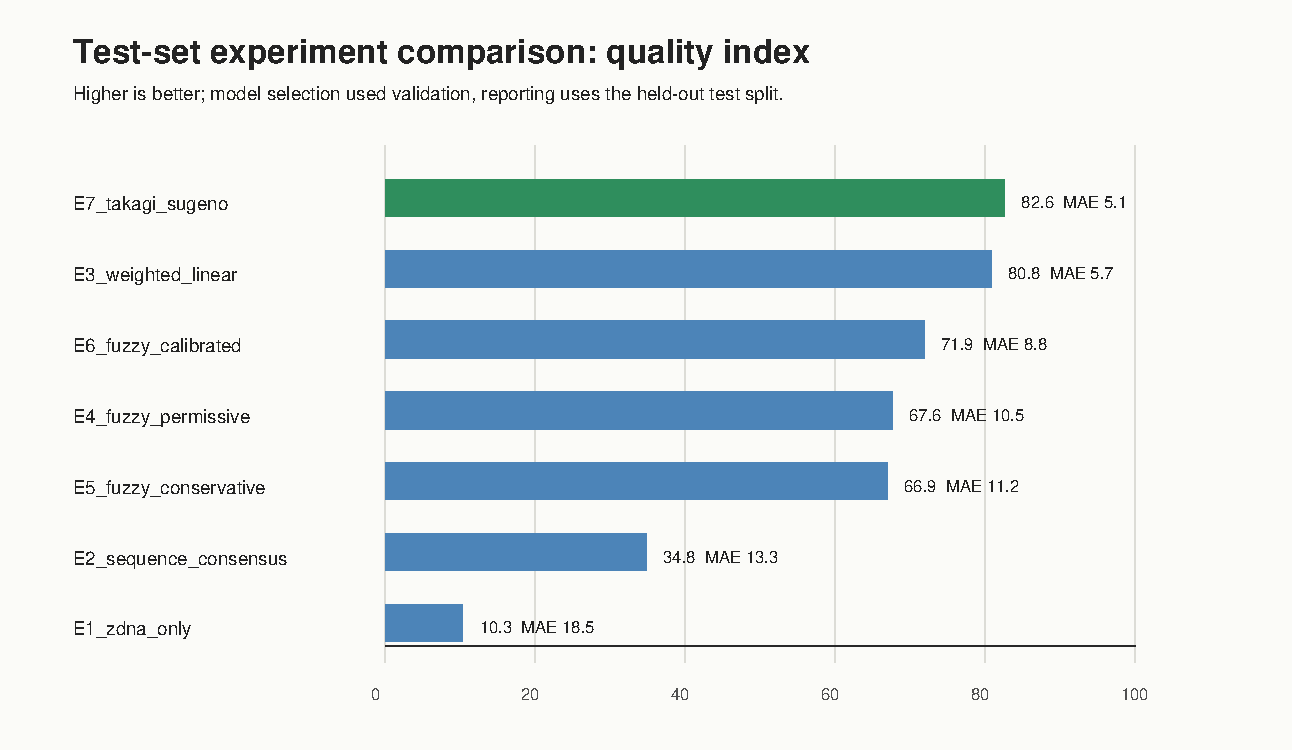
\includegraphics[width=\linewidth]{../outputs/experiment_quality.pdf}
\caption{Porovnanie modelov podľa kompozitného indexu kvality na testovacom splite. Model E7 bol vybraný podľa validačného splitu a dosiahol najlepší testovací index.}
\end{figure}

\begin{figure}[htbp]
\centering
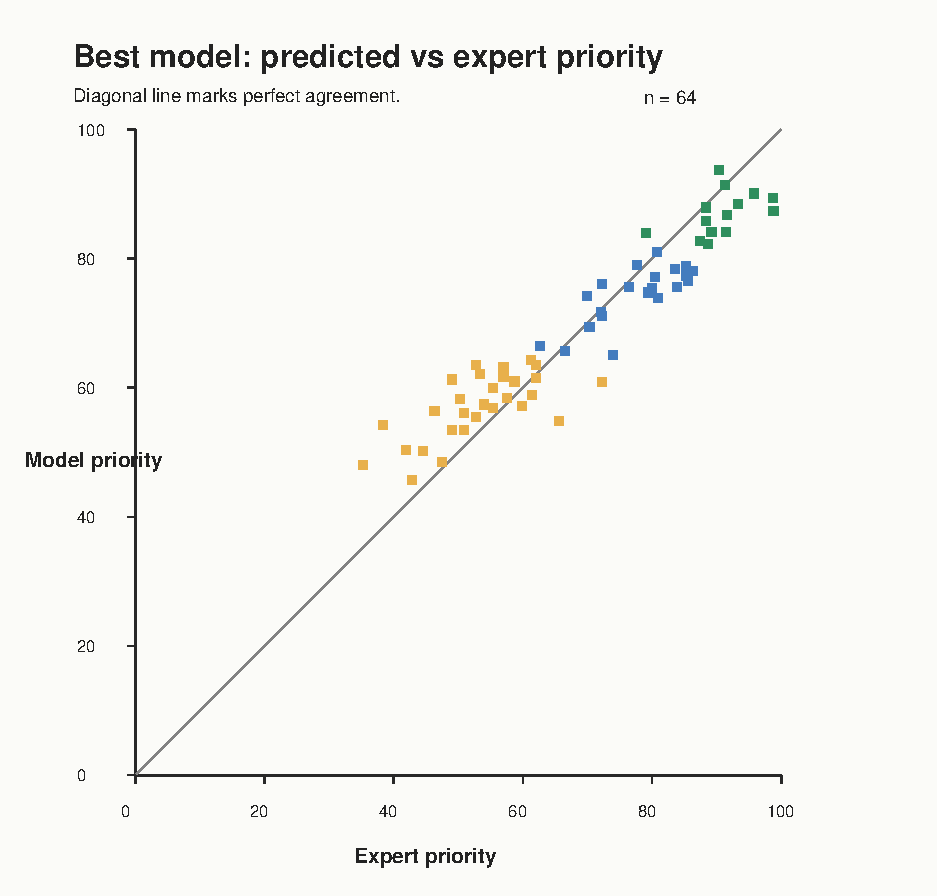
\includegraphics[width=0.82\linewidth]{../outputs/prediction_vs_expert.pdf}
\caption{Vzťah medzi referenčným skóre a skóre vybraného modelu E7 na testovacom splite. Diagonála označuje ideálnu zhodu.}
\end{figure}

Výsledky ukazujú, že samotné \texttt{zdna\_score} nie je vhodné ako rozhodovací model pre validačnú prioritu. Sekvenčný konsenzus zlepšil výber oproti baseline, ale stále ignoroval regulačný kontext a bias. Vážený lineárny model E3 bol silný, no jeho nevýhodou je slabšia pravidlová interpretácia. Čisté Mamdaniho iterácie E4 až E6 boli transparentné, ale pri prísnejších pravidlách strácali numerickú presnosť. Najlepší kompromis dosiahol E7: zachoval fuzzy pravidlá pre lokálne režimy rozhodovania, použil numerické konsekventy vhodné na kalibráciu a po úprave dĺžkového rozsahu 8 až 400 bp dosiahol najvyšší validačný aj testovací index.

\begin{table}[htbp]
\centering
\caption{Najvyššie zoradení kandidáti vybraným modelom E7.}
\small
\begin{tabular}{llrr}
\toprule
Poradie & Kandidát & Model & Referencia \\
\midrule
1 & ZFR\_0127 & 96,1 & 100,0 \\
2 & ZFR\_0311 & 93,7 & 90,4 \\
3 & ZFR\_0041 & 93,1 & 96,7 \\
4 & ZFR\_0018 & 92,4 & 100,0 \\
5 & ZFR\_0105 & 91,9 & 96,3 \\
6 & ZFR\_0207 & 91,7 & 94,6 \\
7 & ZFR\_0319 & 91,4 & 91,3 \\
8 & ZFR\_0225 & 90,9 & 98,5 \\
\bottomrule
\end{tabular}
\end{table}

Audit pokrytia pravidiel kontroluje, či finálny model nepoužíva iba jeden dominantný režim rozhodovania a či lokálne pravidlá E7 reálne prispievajú k rôznym typom kandidátov. Tabuľka nižšie sumarizuje všetky aktívne Takagiho-Sugenove pravidlá na testovacom splite. Pokrytie vyjadruje podiel kandidátov, pri ktorých malo pravidlo nenulovú aktiváciu; priemerná aktivácia ukazuje jeho typickú silu.

\begin{table}[htbp]
\centering
\caption{Rule coverage audit finálneho modelu E7 na testovacom splite.}
\footnotesize
\setlength{\tabcolsep}{4pt}
\begin{tabular}{l>{\raggedright\arraybackslash}p{4.4cm}rr>{\raggedright\arraybackslash}p{3.4cm}}
\toprule
Pravidlo & Úloha pravidla & Pokrytie [\%] & Priem. aktivácia & Dominantná fronta \\
\midrule
TS6 & vyvážený kandidát druhej vlny & 59,38 & 0,407 & C \\
TS10 & silný a dobre validovateľný kandidát & 32,81 & 0,583 & A \\
TS3 & silný signál pri strednom kontexte & 21,88 & 0,350 & B \\
TS4 & kontext kompenzuje stredný signál & 20,31 & 0,373 & A \\
TS1 & silný signál, kontext, evidencia a nízky bias & 14,06 & 0,562 & A \\
TS2 & silný kontext s použiteľnou evidenciou & 14,06 & 0,562 & A \\
TS5 & silný signál bez regulačného kontextu & 14,06 & 0,338 & C \\
TS7 & vysoký bias pri slabšej evidencii & 4,69 & 0,206 & C \\
\bottomrule
\end{tabular}
\end{table}

\section{Ablačná analýza vstupov}

Aby bolo jasné, ktoré vstupy reálne prispievajú k rozhodnutiu, bol vybraný model E7 opakovane vyhodnotený na testovacom splite po odstránení jednej skupiny informácií. Pri odstránení CpX kontextu sa zo skóre regulačného kontextu odpočítala CpX zložka, pri odstránení TSS sa odpočítala TSS zložka, pri odstránení biasu sa riziko biasu neutralizovalo a pri odstránení validovateľnosti sa validovateľnosť nahradila neutrálnou hodnotou.

\begin{table}[htbp]
\centering
\caption{Ablačná analýza vybraného modelu E7 na testovacom splite.}
\small
\begin{tabular}{lrrrr}
\toprule
Scenár & MAE & Fronta & Index & Strata indexu \\
\midrule
Plný model & 5,15 & 0,766 & 82,59 & 0,00 \\
Bez CpX kontextu & 6,02 & 0,719 & 81,90 & 0,69 \\
Bez TSS vzdialenosti & 8,74 & 0,578 & 73,34 & 9,24 \\
Bez biasu & 8,29 & 0,516 & 70,64 & 11,95 \\
Bez validovateľnosti & 6,15 & 0,688 & 78,23 & 4,35 \\
\bottomrule
\end{tabular}
\end{table}

\begin{figure}[htbp]
\centering
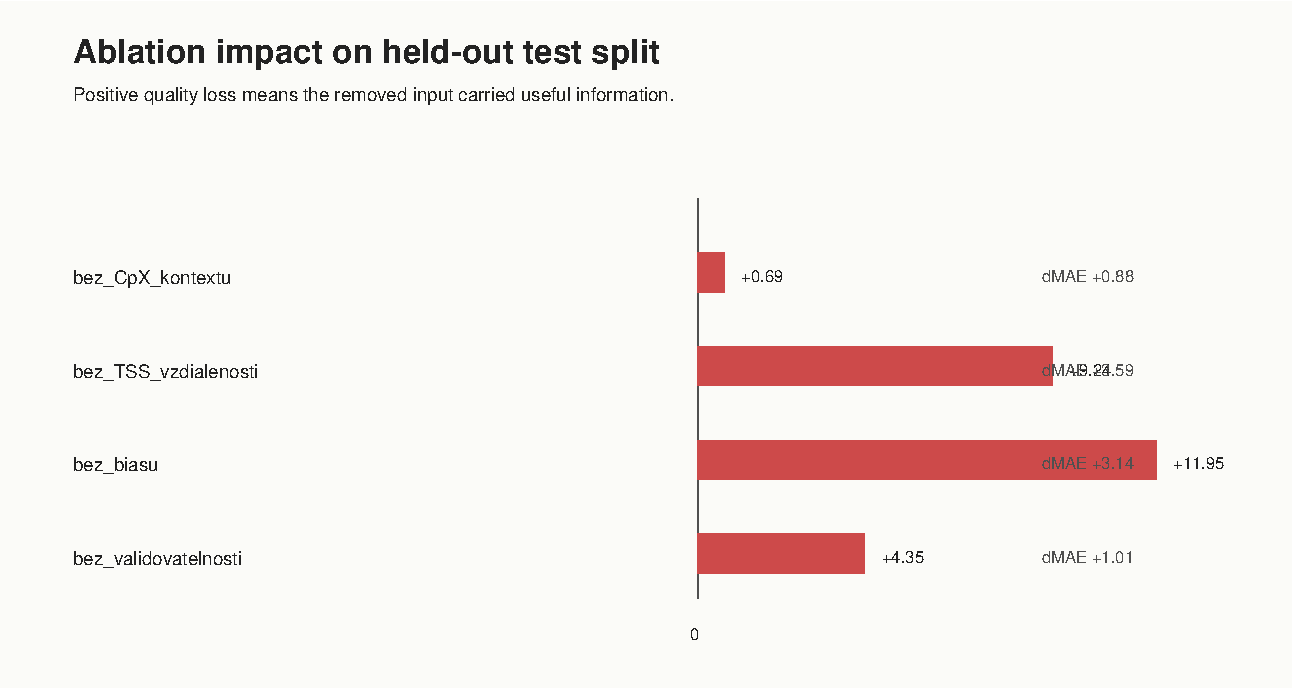
\includegraphics[width=\linewidth]{../outputs/ablation_impact.pdf}
\caption{Dopad ablácií na kompozitný index kvality. Najväčšiu stratu spôsobilo odstránenie TSS vzdialenosti, potom biasu a CpX kontextu.}
\end{figure}

Najsilnejší prínos mal bias a TSS vzdialenosť. Odstránenie biasu znížilo index kvality o 11,95 bodu, pretože bez explicitnej penalizácie repetitívnosti a proxy evidencie model presúva rizikové kandidáty do príliš vysokej priority. Odstránenie TSS vzdialenosti zvýšilo MAE z 5,15 na 8,74 a znížilo presnosť fronty z 0,766 na 0,578. Validovateľnosť mala stredný vplyv a pomáhala pri rozhodovaní okolo hranice front \texttt{A} a \texttt{B}. CpX kontext bol v hlavnom benchmarku prínosný, ale po skrátení dĺžkového rozsahu mal menší samostatný efekt než TSS a bias.

\section{Intervalová neistota}

Intervalová neistota bola odhadnutá opakovaným behom modelu E7 s perturbovanými vstupmi. Pri každom testovacom kandidátovi sa 80-krát mierne zmenilo sekvenčné skóre, sekvenčná pravdepodobnosť, CpX prekryv, TSS vzdialenosť, repetitívny prekryv, unikátnosť primerov a dĺžka regiónu. Výsledkom je interval medzi 5. a 95. percentilom skóre priority.

\begin{figure}[htbp]
\centering
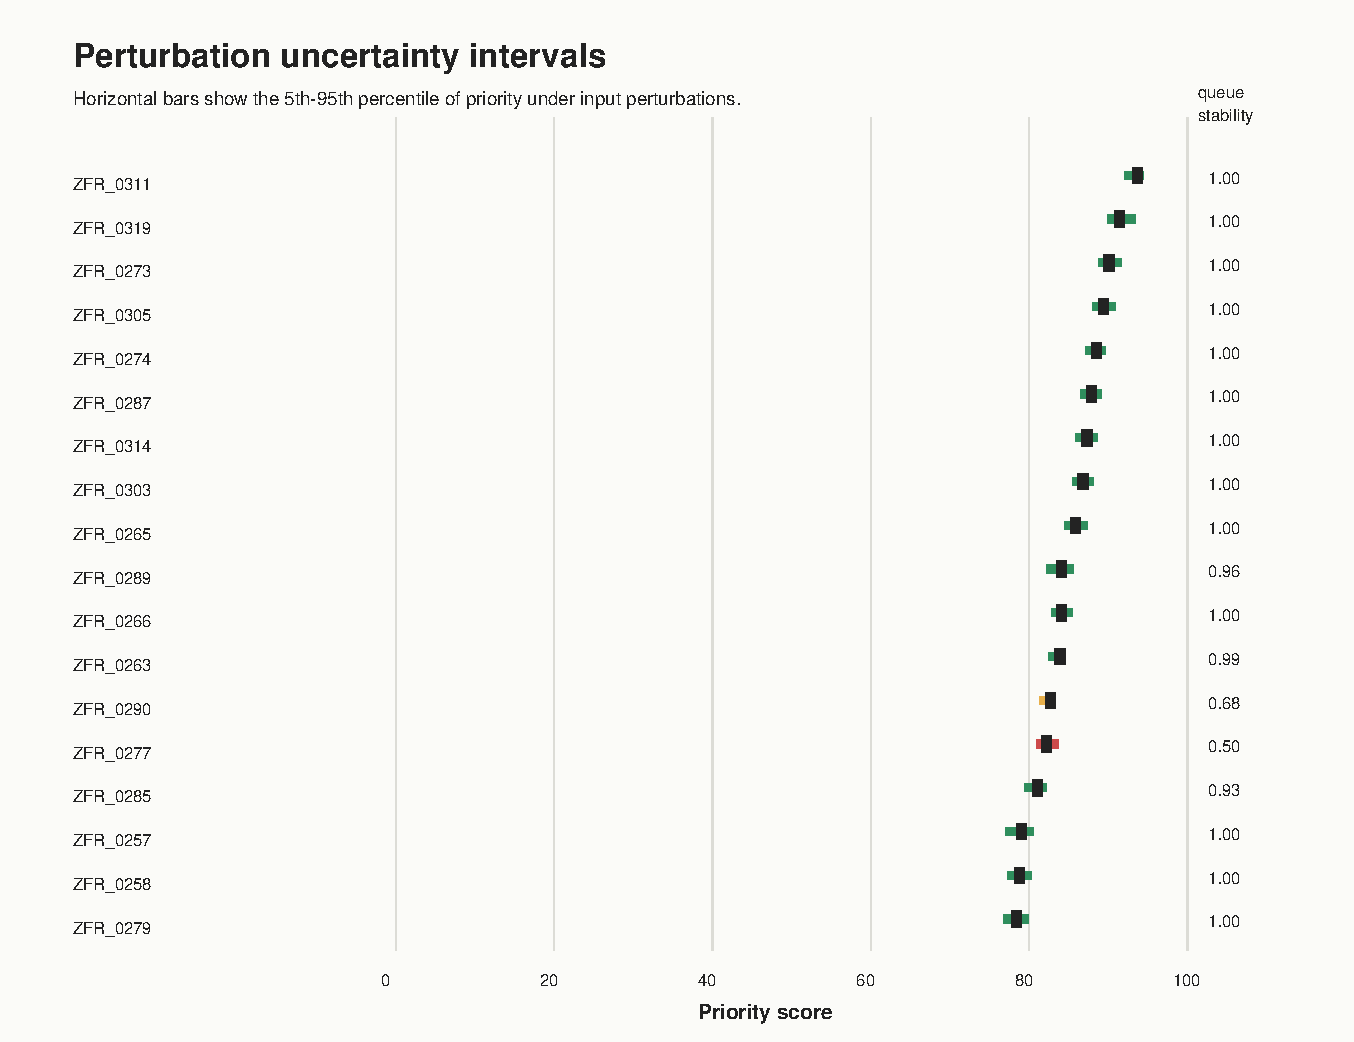
\includegraphics[width=\linewidth]{../outputs/uncertainty_intervals.pdf}
\caption{Intervaly neistoty pre najvyššie prioritizované testovacie kandidáty. Čierny bod označuje základné skóre, farebný interval 5. až 95. percentil a pravý stĺpec stabilitu rozhodovacej fronty.}
\end{figure}

Priemerná šírka 5--95\% intervalu bola 2,99 bodu a priemerná stabilita rozhodovacej fronty 0,962. Najvyššie prioritizované kandidáty mali úzke intervaly a stabilitu blízku 1,0. Nižšia stabilita sa objavovala najmä pri kandidátoch tesne pri hranici front, kde malá zmena vstupu mohla presunúť kandidáta medzi \texttt{A\_validovat} a \texttt{B\_prioritne\_preskumat}. Takýto kandidát by v praxi nemal byť zamietnutý automaticky; vhodnejšia je manuálna kontrola alebo opätovné prepočítanie po doplnení anotácií.

\section{Externé overenie na Shin dátach}

Ako externá kontrola bol pripravený Shin validačný dataset z reálnych per-locus overlay súborov. Dataset obsahuje 312 experimentálne pozitívnych a 73 experimentálne negatívnych intervalov zo Shin et al. \citep{shin2016}. Každý interval bol prepočítaný na kandidáta podľa dostupných prekryvov so Z-DNA Hunter výstupmi modelu 1 a modelu 2. Kandidátna dĺžka bola odvodená z najsilnejšieho reálneho prekryvu a obmedzená na rozsah 8 až 400 bp, aby zodpovedala rozsahu hlavného rozhodovacieho modelu a zároveň pokryla 384 bp Shin lokusy. Pole \texttt{z\_dnabert\_probability} je v tomto overení prázdne, takže výpočet \texttt{z\_signal} používa iba Hunter-derived \texttt{zdna\_score}.

Kalibrácia Shin vstupu prebehla v troch iteráciách. Prvá varianta použila iba tri model2 nastavenia a správala sa podobne ako jednoduchý citlivostný filter. Druhá varianta pridala \texttt{model1\_10bp}, čím vznikol nezávislý hlas modelovej rodiny 1 a pravidlo \texttt{cross\_tool}. Finálna varianta doplnila prísnejší \texttt{model2\_8bp\_65perc}; vážený Hunter signál preto kombinuje citlivé \texttt{model2\_8bp} s konzervatívnejšími prahmi \texttt{model1\_10bp}, \texttt{model2\_10bp}, \texttt{model2\_8bp\_65perc} a \texttt{model2\_10bp\_60perc}. Váhy boli nastavené na 0,55, 0,15, 0,10, 0,10 a 0,10 v rovnakom poradí podľa empirického kompromisu recall/špecificita. Pre každý lokus boli súčasťou vstupu aj CpX prekryv, vzdialenosť od TSS zo SGA anotácie, promótorový príznak a počet regulačných značiek. Tieto premenné určujú regulačný kontext, zatiaľ čo sekvenčná zložka zostáva založená výhradne na Z-DNA Hunter výstupoch.

\begin{table}[htbp]
\centering
\caption{Binárne porovnanie na reálnych Shin overlay dátach.}
\footnotesize
\setlength{\tabcolsep}{4pt}
\begin{tabular}{>{\raggedright\arraybackslash}p{4.8cm}rrrrr}
\toprule
Model alebo prah & Recall & Specificity & Balanced acc. & 95\% CI & Youden J \\
\midrule
ZDNABERT HG18 th 0.25 & 0,877 & 0,890 & 0,880 & 0,842--0,923 & 0,770 \\
Z-DNA Hunter model 2 size 10 & 0,726 & 0,973 & 0,850 & 0,817--0,880 & 0,700 \\
Z-DNA Hunter model 2 size 8 & 0,822 & 0,849 & 0,840 & 0,787--0,879 & 0,670 \\
E7, prah \texttt{A\_validovat} & 0,369 & 0,986 & 0,677 & 0,646--0,707 & 0,355 \\
E7, prah \texttt{B\_prioritne\_preskumat} & 0,811 & 0,836 & 0,823 & 0,773--0,869 & 0,647 \\
E7, Z-DNA Hunter + fuzzy prah 67,5 & 0,772 & 0,932 & 0,852 & 0,814--0,888 & 0,704 \\
\bottomrule
\end{tabular}
\end{table}

\begin{table}[htbp]
\centering
\caption{Konfúzna matica Shin validácie pre Z-DNA Hunter + E7 fuzzy vrstvu pri prahu 67,5.}
\small
\begin{tabular}{lrr}
\toprule
Skutočný stav & Predikované pozitívne & Predikované negatívne \\
\midrule
Experimentálne pozitívne & 241 & 71 \\
Experimentálne negatívne & 5 & 68 \\
\bottomrule
\end{tabular}
\end{table}

Citlivejšia validácia pravidiel nehodnotila iba pevné hranice front \texttt{A}, \texttt{B} a \texttt{C}. Nad Shin predikciami bol urobený prahový sweep v rozsahu 0 až 100 bodov s krokom 0,5 a pre každý prah sa prepočítal recall, špecificita, balanced accuracy a Youdenov index. Pevný prah \texttt{A\_validovat} testuje konzervatívnosť prvej validačnej fronty, prah \texttt{B\_prioritne\_preskumat} testuje použiteľnosť širšieho výberu kandidátov a prah 67,5 ukazuje najlepší operačný kompromis na externých Shin dátach. Tento postup nemení pravidlovú bázu; slúži ako citlivejšia kontrola toho, ako stabilne sa spojité fuzzy skóre správa pri binárnom validačnom rozhodnutí.

\begin{figure}[htbp]
\centering
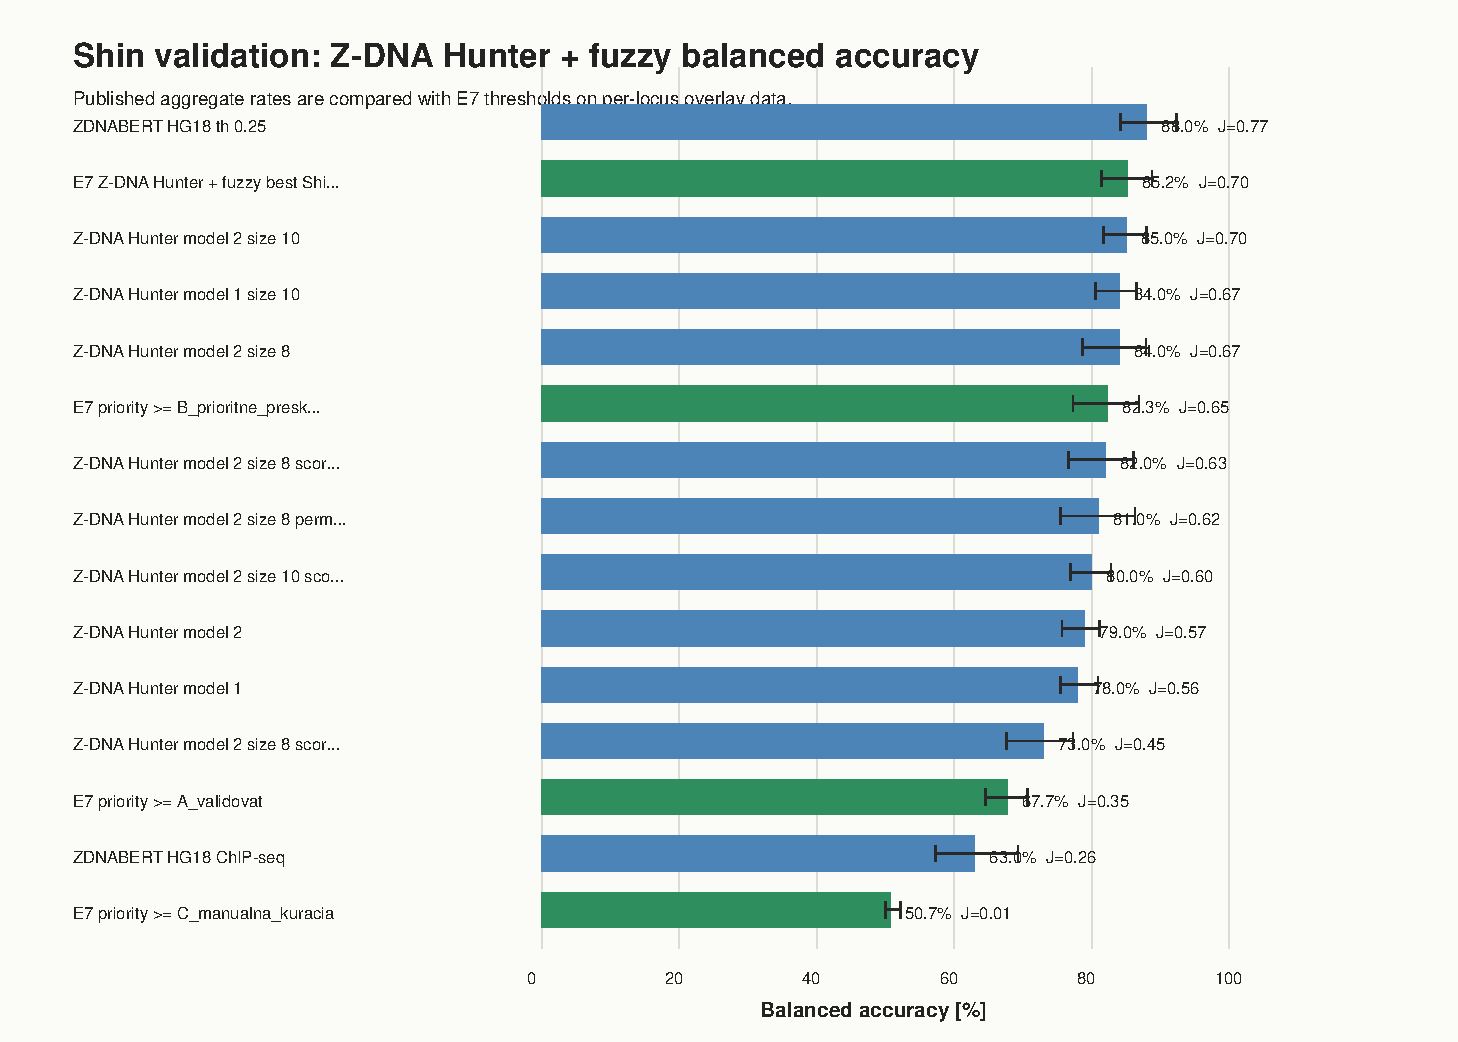
\includegraphics[width=\linewidth]{../outputs/shin_real_comparison.pdf}
\caption{Porovnanie vybraného E7 modelu s agregovanými výsledkami Z-DNA Hunter a ZDNABERT na reálnych Shin overlay dátach. Zelené stĺpce označujú prahy rozhodovacieho modelu; ZDNABERT je iba externá referencia a nebol použitý pri výpočte E7 vstupov.}
\end{figure}

\begin{figure}[htbp]
\centering
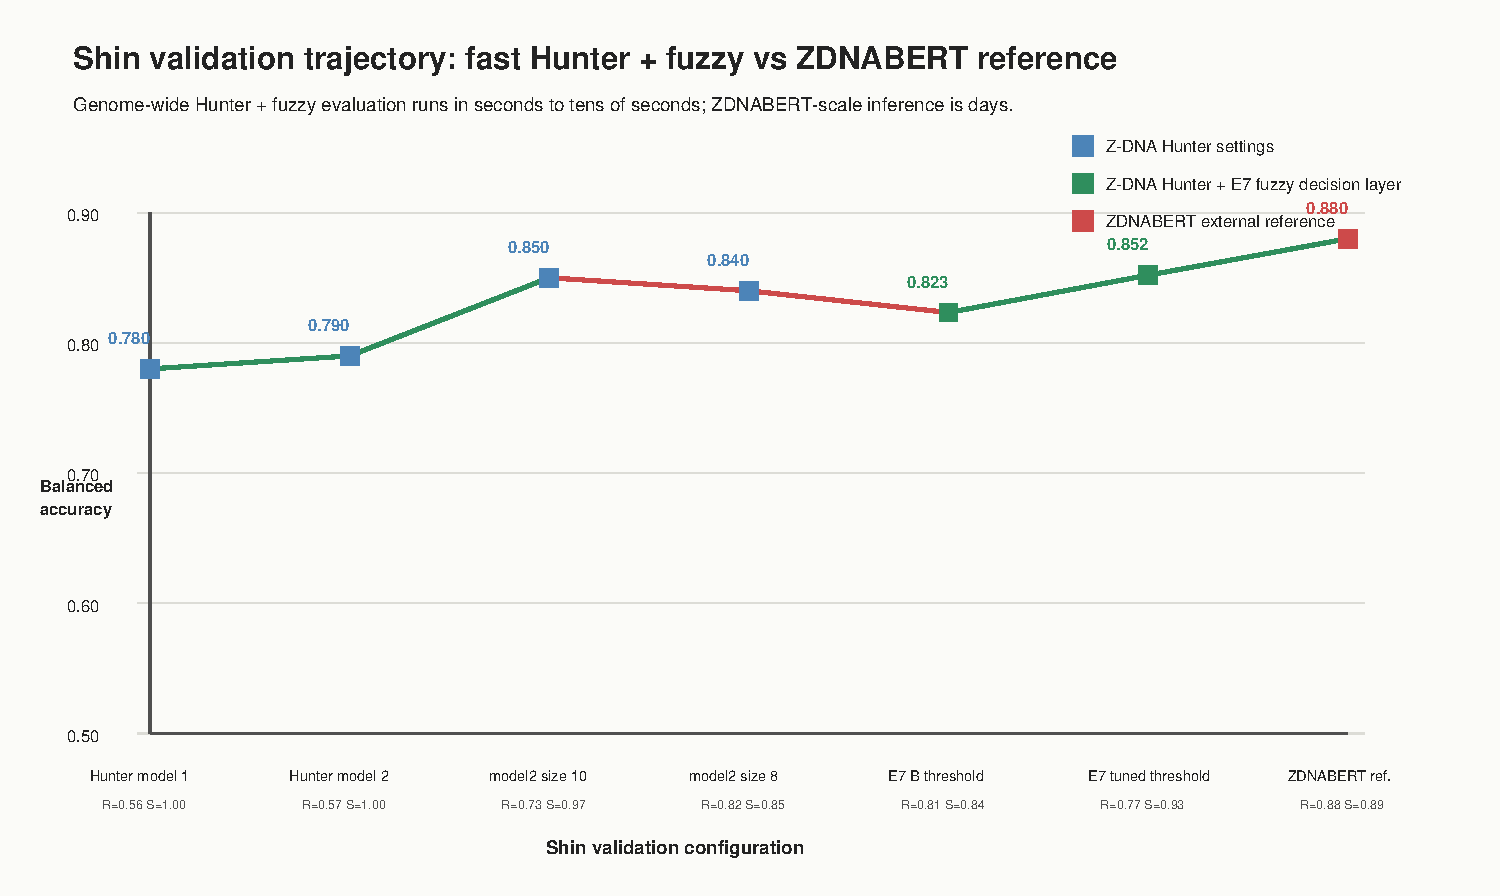
\includegraphics[width=\linewidth]{../outputs/shin_validation_trajectory.pdf}
\caption{Trajektória zlepšenia a zhoršenia balanced accuracy pri Shin validácii. Modré body sú samostatné Z-DNA Hunter nastavenia, zelené body sú rozhodnutia Z-DNA Hunter + E7 fuzzy vrstvy a červený bod je externá ZDNABERT referencia.}
\end{figure}

Intervaly spoľahlivosti v tabuľke boli odhadnuté bootstrapom nad Shin lokusmi. Pri prísnom prahu \texttt{A\_validovat} bol model veľmi konzervatívny: zachytil 115 z 312 pozitívnych intervalov a zaradil iba jeden negatívny interval do prvej validačnej fronty. Pri prahu \texttt{B\_prioritne\_preskumat} alebo vyššie dosiahol recall 0,811, špecificitu 0,836 a balanced accuracy 0,823. Najlepší binárny prah Z-DNA Hunter + fuzzy vrstvy bol 67,5 bodu; pri ňom model dosiahol recall 0,772, špecificitu 0,932, balanced accuracy 0,852 a Youdenov index 0,704. Graf ukazuje, že citlivejšie Hunter nastavenie zlepšilo recall, ale zhoršilo špecificitu; fuzzy nadstavba potom časť tejto straty kompenzovala a posunula výsledok späť k vyváženejšiemu rozhodnutiu. V dostupných per-locus súboroch tým zlepšila samostatné reálne overlay vstupy \texttt{model2\_10bp} (balanced accuracy 0,824) a \texttt{model2\_8bp} (0,791). Jej 95\% interval balanced accuracy 0,814--0,888 sa zároveň prekrýva so ZDNABERT referenciou 0,842--0,923, hoci ZDNABERT nebol použitý ako vstup modelu.

Praktický význam je najmä výpočtový. Merací protokol celogenómového behu Z-DNA Hunter je uvedený v práci Petrovič et al. \citep{petrovic2025}. Fuzzy nadstavba pracuje nad hotovými kandidátmi, takže na celogenómovej úrovni pridáva iba rýchle tabuľkové pravidlové vyhodnotenie v rozsahu niekoľkých sekúnd až desiatok sekúnd. ZDNABERT-like prístup pri celogenómovom použití typicky znamená niekoľko dní výpočtu. Výsledok preto podporuje použitie E7 ako rýchlej nadstavby nad Z-DNA Hunter, ktorá je na Shin validácii porovnateľná so ZDNABERT referenciou v balanced accuracy a zároveň ostáva interpretovateľná pravidlovou bázou.

\section{Validácia a verifikácia}

Verifikácia systému znamená kontrolu, či implementácia zodpovedá navrhnutým pravidlám. Skript preto pri každom kandidátovi zapisuje najaktívnejšie pravidlá do \path{outputs/rules_audit.txt}. Kandidát s vysokým \texttt{z\_signal}, vysokým regulačným kontextom, silnou evidenciou a vysokou validovateľnosťou aktivuje pravidlá pre vysokú prioritu. Kandidát s vysokým rizikom repetitívnosti aktivuje pravidlá znižujúce dôveryhodnosť evidencie.

Validácia systému znamená posúdenie, či odporúčania dávajú biologický a metodický zmysel. Pri ďalšom rozšírení by bolo vhodné porovnať odporúčania so Z-DNA ChIP-seq dátami \citep{shin2016}, mapovaním jednoreťazcovej DNA pomocou KAS-seq \citep{wu2020}, prípadne širším non-B DNA mapovaním \citep{kouzine2017}. Doplnkovým referenčným zdrojom môže byť databáza non-B DNA motívov \citep{cer2013}. Dôležité je vyhnúť sa kruhovej validácii: úspech modelu nemožno dokazovať iba tým istým skóre, ktoré bolo použité ako vstup.

\section{Ďalšie možné vylepšenia}

V ďalšej iterácii by bolo možné:

\begin{itemize}
  \item kalibrovať funkcie príslušnosti pomocou panelu viacerých expertov a sledovať medziexpertnú zhodu,
  \item optimalizovať parametre fuzzy množín pomocou validačného splitu, ale zachovať obmedzenia interpretovateľnosti,
  \item pridať samostatnú triedu pre kandidátov na antisense alebo intragénnych pozíciách, ak budú biologicky relevantné,
  \item rozšíriť neistotu aj na neistotu anotácie TSS a CpX ostrovčekov, nielen na numerickú perturbáciu,
  \item porovnať E7 s neuro-fuzzy modelom, ktorý by sa učil pravidlá automaticky, a následne porovnať jeho interpretovateľnosť s ručne navrhnutou bázou,
  \item rozšíriť Shin overenie o ďalšie regulačné a bunkovo špecifické anotačné vrstvy,
  \item testovať model na nezávislých experimentálnych dátach z ďalších druhov.
\end{itemize}

\section{Diskusia}

Navrhnutý systém má tri praktické výhody. Prvou je interpretovateľnosť: každé rozhodnutie možno spätne vysvetliť aktivovanými pravidlami alebo lokálnymi Takagiho-Sugenovými konsekventmi. Druhou je modularita: vstupné sekvenčné skóre môže pochádzať z heuristického nástroja alebo zo sekvenčného modelu bez zmeny rozhodovacej vrstvy. Treťou je metodická opatrnosť: systém explicitne penalizuje bias a neinterpretuje samotnú sekvenčnú predispozíciu ako dôkaz funkčnej Z-DNA aktivity.

Porovnanie modelov ukazuje aj dôležitý metodický detail. Čisto interpretovateľný Mamdaniho model je vhodný na vysvetľovanie, ale pri spojitom prioritizačnom skóre môže byť menej presný. Vážený lineárny model je presný, ale neponúka pravidlové vysvetlenie. Takagiho-Sugenov model E7 predstavuje kompromis: zachováva pravidlové lokálne režimy, ale numerické konsekventy umožňujú lepšie doladenie skóre.

\section{Záver}

Seminárna práca navrhla a implementovala univerzálny rozhodovací systém pre prioritizáciu Z-DNA-formujúcich regiónov v genómových dátach. Riešenie používa normalizovaný vstup \texttt{zdna\_score}, sekvenčný modelový signál, regulačný kontext, typ evidencie, bias a praktickú validovateľnosť. Experimentálne porovnanie siedmich stratégií ukázalo, že najlepší kompromis medzi presnosťou a interpretovateľnosťou dosiahol Takagiho-Sugenov fuzzy model E7. Ablácia potvrdila prínos TSS vzdialenosti, biasu, CpX kontextu a validovateľnosti. Perturbačná analýza doplnila intervalovú neistotu a Shin kontrola na reálnych Z-DNA Hunter overlay dátach ukázala, že model pri externom binárnom prahu 67,5 bodu dosahuje balanced accuracy 0,852 s 95\% intervalom 0,814--0,888 a zachováva vysokú špecificitu voči experimentálne negatívnym kandidátom.

\bibliographystyle{plainnat}
\bibliography{references}

\end{document}
